\subsection{Интернет вещей}
\label{sec:subject:iot}

Интернет вещей — концепция вычислительной сети физических предметов («вещей»), оснащённых встроенными технологиями для взаимодействия друг с другом или с внешней средой, рассматривающая организацию таких сетей как явление, способное перестроить экономические и общественные процессы, исключающее из части действий и операций необходимость участия человека \cite{wiki_iot}.

Концепция сформулирована в 1999 году как осмысление перспектив широкого применения средств радиочастотной идентификации для взаимодействия физических предметов между собой и с внешним окружением. Наполнение концепции «интернета вещей» многообразным технологическим содержанием и внедрение практических решений для её реализации начиная с 2010-х годов считается устойчивой тенденцией в информационных технологиях, прежде всего, благодаря повсеместному распространению беспроводных сетей, появлению облачных вычислений, развитию технологий межмашинного взаимодействия, началу активного перехода на IPv6[4] и освоению программно-конфигурируемых сетей \cite{wiki_iot}.

На 2017 год термин «Интернет вещей» распространяется не только на киберфизические системы для «домашнего» применения, но и на промышленные объекты. Развитие концепции «Интеллектуальных зданий» получило название «Building Internet of Things» (BIoT, «Интернет вещей в здании»), развитие распределённой сетевой инфраструктуры в АСУ ТП привело к появлению «Industrial Internet of Things» (IIoT, «Индустриальный (промышленный) интернет вещей») \cite{wiki_iot}.

Что представляет из себя интернет вещей:
\begin{itemize}
	\item постоянная поддержка человека предметами, которые его находятся рядом с ним;
	\item прозрачность процессов, ориентация на результат;
	\item это говорить не как надо делать, а что должно получиться.
\end{itemize}

Интернет вещей (IoT) – это, в основном, физические устройства: транспортные средства, бытовая техника, строительные материалы и другие предметы, взаимосвязанные между собой с целью сбора и обмена данными при помощи датчиков, программного обеспечения, проводов, микрочипов и прочей электроники через подключение к Сети (Интернет, Bluetooth).

Самоуправляемые автомобили, личные помощники, бытовая смарт-техника, энергосберегающие строительные материалы – этот список можно продолжать бесконечно. Все это влияющие на массы продукты, которые разрабатываются и развиваются для того, чтобы сделать жизнь проще, функциональнее, продуктивнее и эффективнее.

Согласно исследованиям компании Gartner, к прошлому году существовало 3.8 миллиардов соединенных между собой устройств: смарт-автомобили, детекторы дыма, дверные замки, промышленные роботы, уличные фонари, программы для мониторинга сердечного ритма, поезда, ветровые турбины, даже теннисные ракетки и тостеры.

По подсчетам компании, к 2020 г будет существовать 25 миллиардов смарт-девайсов, передающих крошечные объемы информации нам, в облако и обратно. Уходящий в отставку генеральный директор Cisco Джон Чамберс заявил, что в течение 5 лет будут существовать 50 миллиардов девайсов на сумму 19 триллионов долларов США. Говорят, что эти смарт-девайсы начинают приводить в действие четвертую промышленную революцию (после пара, электричества и проводных компьютеров).

~
\begin{figure}[H]
\centering
	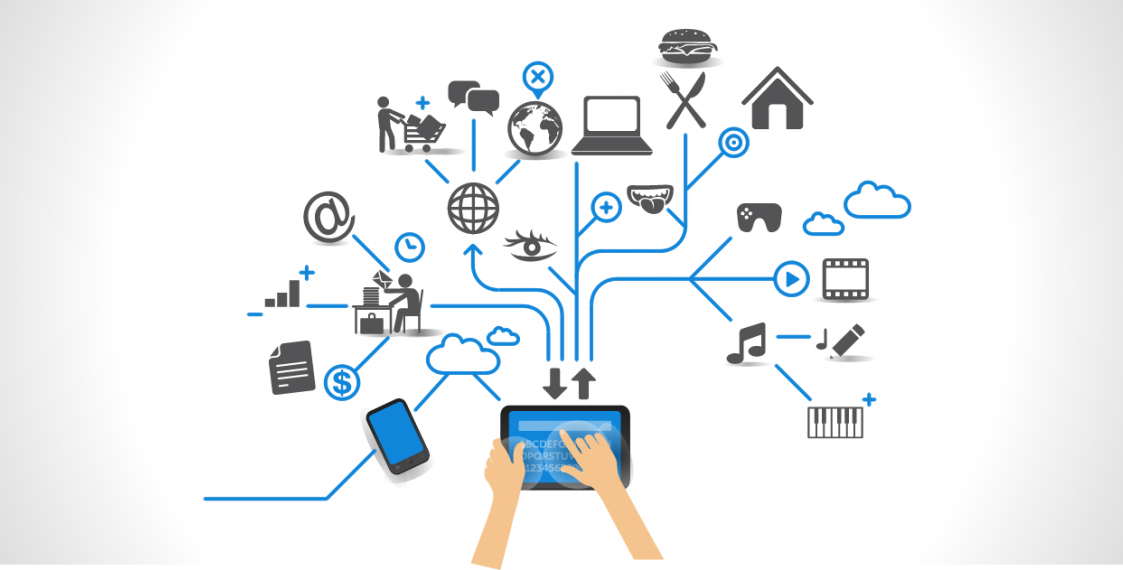
\includegraphics[scale=0.4]{figures/iot_scheme.png}
	\caption{Схематичное представление IoT}
	\label{fig:subject:iot:scheme}
\end{figure}

4 примера умных интернет вещей:
\begin{itemize}
	\item если вы уйдете из дома без кошелька, он сообщит вам об этом по телефону, а сенсор на ошейнике кота сообщит координаты,если кот сбежал далеко от дома;
	\item если вы забыли выключить утюг или телевизор, не нужно идти домой проверять: они сами доложат свой статус;
	\item когда закончился кофе или стиральный порошок, заказать его можно одним нажатием на кнопку;
	\item интернет-вещи напомнят, когда нужно поливать цветы, а целая система, подключенная к вашему огороду, подскажет, когда нужно полить грядки и включить поливающее оборудование;
\end{itemize}

Наше световое оборудование, поставляемое вместе с мобильным приложением, как раз подходит под описание интернета вещей. Данные устройства (гирлянды), обладают wi-fi модулями для связи с мобильны приложением и получением команд от него, а также для связи с другими гирляндами. Само приложение обладает возможностью объединения гирлянд в группы, для последующего взаимодействия сразу с несколькими гирляндами (например при внешнем украшении дома). 

Мобильное приложение~--- программное обеспечение, предназначенное для работы на смартфонах, планшетах и других мобильных устройствах. Многие мобильные приложения предустановлены на самом устройстве или могут быть загружены на него из онлайновых магазинов приложений, таких как App Store, BlackBerry App World, Google Play, 1mobile market, Windows Phone Store, Яндекс.store и других, бесплатно или за плату \cite{wiki_mobile_def}.

На сегодняшний день существует огромное количество разнообразных приложений, загружаемых в мобильный телефон. Все приложения можно условно разделить на развлекательные (игры, плееры, «читалки»), коммуникационные (мессенджеры, навигационные (карты), справочные (словари, базы данных) и прикладные (все от калькулятора до графических программ) \cite{mobile_business}.

Мобильные технологии имеют ряд неоспоримых преимуществ перед любыми другими видами маркетинговых коммуникаций. Использование в своем приложении функций игрового характера позволяет привлечь большую аудиторию, заинтересовав ее. Вы можете получать отзывы напрямую от своих клиентов, без посредников (таких, как интернет-сайты или ваши сотрудники) и прямо в момент совершения покупки.

Возможности мобильных приложений практически безграничны, но немало программ удаляются пользователем уже через пару суток после установки. Так что к разработке мобильного приложения стоит относиться серьезно и ответственно, как и к любому другому инструменту маркетинга.

В 2012 году рынок мобильных приложений оценивался в 53 миллиарда долларов, а прогноз на 2016 год гласил, что предполагаемый рост составит около 100 миллиардов долларов. Эти цифры немного отличаются у разных исследователей, но очевидным остается то, что мобильный рынок действительно масштабен. Доход разработчики получают с помощью внутренних in-app покупок, рекламы внутри приложений, а также сбора больших данных (big data). Самые многообещающие категории – это социальные сети, производительность, рекламные сервисы, а также полезные приложения для различных целей. Самые быстрорастущие рынки – Юго-Восточная Азия и Латинская Америка \cite{mobile_market}.

В США, 67~\% пользователей используют смартфон, чтобы выходить в интернет каждый день, и большинство никогда не выйдут из дома без своего телефона. Аналогичный рост использования смартфонов наблюдается и в России – даже пользователи с доходами ниже среднего чаще выбирают смартфон вместо компьютера, чтобы всегда оставаться на связи с миром. Исследования рынка показывают, что около половины всех пользователей мобильных телефонов загрузили приложения, а две трети из них регулярно их используют. Большинство пользователей мобильных приложений находятся в возрастном промежутке от 25 до 30 лет, женаты или замужем, живут в пригородных районах, и имеют высшее образование. Таким образом, пользователи мобильных приложений в целом моложе, более образованы и имеют более высокий доход, нежели пользователи, не использующие мобильные приложения \cite{mobile_market}.

Две операционные системы Android и iOS доминируют на мобильном рынке. У Apple и Google два самых популярных магазина приложений, и сегодня кажется, что другим участникам рынка можно даже не мечтать, чтобы пробиться к лидерству.

Есть интересная статистика среднемесячного дохода, который приносили мобильные приложения. Статистику привел иностранный Forbes. Итак, в 2013-м году iOS приносила своим разработчикам в среднем \$4 000 в месяц, на втором месте был Android с его \$1 125, и аутсайдером был Windows Phone и всего \$625 \cite{mobile_tendency}.

В 2016-м году ситуация поменялась. Согласно данным Statista, приложение Windows Phone приносит, в среднем, \$11 400 в месяц, тогда как приложение iOS генерирует \$8 100, а Android — \$4 900. При этом 75~\% разработчиков являются приверженцами Android \cite{mobile_tendency}.

Все это говорит нам о том, что рынок мобильных приложений является очень перспективным и быстрорастущим. Мобильные приложения очень помогают в продвижении товара. Также они очень удобны как для пользователя, так и для разработчика, так как предоставляют большой спектр всевозможных датчиков и сетевых возможностей. Теперь понятно, что управление световым оборудованием с помощью именно мобильного приложения, это самый логичный и верный вариант для выбора вектора развития производства светового оборудования.